\documentclass[11pt,letterpaper]{article}

% ------------------------------------------------------------
% Paquetes
% ------------------------------------------------------------
\usepackage[spanish,provide=*]{babel}
\usepackage[utf8]{inputenc}
\usepackage[T1]{fontenc}
\usepackage[margin=2.5cm]{geometry}
\usepackage{tikz}
\usepackage{float}
\usetikzlibrary{shapes.multipart,arrows.meta,positioning,fit,backgrounds,calc}
\usepackage{booktabs}
\usepackage{longtable}
\usepackage{array}
\usepackage{enumitem}
\usepackage{hyperref}
\usepackage{xcolor}
\usepackage{titlesec}
\usepackage{fancyhdr}
\usepackage{parskip}

\hypersetup{
  colorlinks=true,
  linkcolor=black,
  urlcolor=blue!50!black,
  citecolor=black,
  pdftitle={Chat multiusuario en red local},
  pdfauthor={Rocha Haro Cesar Antonio}
}

\definecolor{cajamodelo}{RGB}{223,240,255}
\definecolor{cajacontrol}{RGB}{255,236,210}
\definecolor{cajavista}{RGB}{223,255,224}
\definecolor{cajacomun}{RGB}{240,230,255}
\definecolor{cajaproblema}{RGB}{255,214,214}

\setlength{\headheight}{14pt}
\pagestyle{fancy}
\fancyhf{}
\rhead{Chat multiusuario en red local}
\lhead{Modelado y Programación}
\cfoot{\thepage}

\titleformat{\section}{\Large\bfseries}{\thesection.}{0.5em}{}
\titleformat{\subsection}{\large\bfseries}{\thesubsection}{0.5em}{}

% Caja de "clase" tipo UML simplificada.
% #1 = nombre del nodo (para referenciarlo en \draw)
% #2 = color de relleno
% #3 = ancho del texto
% #4 = opciones extra de posicionamiento (p. ej. "below=1cm of Otro"), puede ir vacío
% Después de la llamada debe seguir, entre llaves, el contenido del nodo.
\newcommand{\classbox}[4]{%
  \node[rectangle split, rectangle split parts=2, draw=black, thick,
        rounded corners=1pt, align=left, font=\footnotesize\ttfamily,
        text width=#3, fill=#2, inner sep=4pt, #4] (#1) }

\title{\textbf{Chat multiusuario en red local}\\[0.3em]
  \large Diseño e implementación de un protocolo cliente-servidor con\\
  programación concurrente, hilos de ejecución y sockets}
\author{Estudiante del curso \emph{Modelado y Programación}\\ \small(Rocha Haro Cesar Antonio)}
\date{\today}

\begin{document}

\maketitle
\thispagestyle{empty}
\tableofcontents
\newpage

% ==============================================================
\section{Resumen}
% ==============================================================

Este proyecto resuelve el problema de conectar a múltiples usuarios dentro
de una red local para que puedan comunicarse mediante mensajes de texto,
siguiendo al pie de la letra un protocolo de aplicación basado en JSON
proporcionado por el profesor del curso. Para lograrlo se construyó un
sistema cliente-servidor: un servidor que acepta conexiones TCP y atiende a
cada cliente en un hilo de ejecución independiente, sincronizando el acceso
al estado compartido (usuarios, salas y sus membresías) mediante exclusión
mutua; y un cliente de consola que se conecta al servidor, envía comandos
del protocolo y muestra en tiempo real lo que otros usuarios van
publicando. Ambos programas se diseñaron siguiendo el patrón
Modelo-Vista-Controlador. El proyecto tuvo dos iteraciones: una primera
versión del servidor escrita en C, que sirvió para entender a fondo el
problema pero que se abandonó por las dificultades de simular
orientación a objetos, manejar memoria manualmente y sincronizar hilos con
mutex de bajo nivel; y una segunda versión, la que finalmente se entrega,
escrita íntegramente en C\# sobre .NET, usando \texttt{System.Text.Json}
para el formato del protocolo. El resultado es un chat funcional que
soporta identificación de usuarios, cambios de estado, mensajes públicos y
privados, y salas privadas con invitación, todo de acuerdo con lo
especificado en el protocolo.

% ==============================================================
\section{Introducción}
% ==============================================================

El problema central que resuelve este proyecto es, en su forma más simple,
\textbf{¿cómo conectar a múltiples personas dentro de una red local para que
puedan intercambiar mensajes de texto entre sí?} Al tratarse de una red
local (y no de Internet abierto), el problema encaja de inmediato en un
problema clásico de redes de cómputo resuelto con \emph{sockets}: un
programa servidor escucha en un puerto conocido y los clientes se conectan
a él.

En el análisis inicial del problema surgieron, en orden, las siguientes
preguntas guía —numeradas aquí porque se retoman más adelante en la sección
de Análisis y Diseño—:

\begin{enumerate}[leftmargin=2.2em]
  \item ¿Cómo conectamos a múltiples personas en una red?
  \item Dado que habrá múltiples usuarios conectados, ¿cómo se va a lidiar
        con todos ellos al mismo tiempo?
  \item ¿La comunicación será directamente entre los clientes?
  \item ¿O habrá un intermediario (el servidor) que reenvíe los mensajes a
        los usuarios correspondientes?
  \item Si hay múltiples usuarios modificando el mismo estado compartido,
        ¿qué sucede si dos de ellos piden acceder al mismo lugar en memoria
        al mismo tiempo?
  \item ¿A cuál de los dos se le da prioridad?
  \item ¿Qué pasa si un usuario elimina cierta información (por ejemplo, al
        desconectarse) justo cuando otro usuario la está solicitando?
  \item ¿Cómo se entera ese segundo usuario de que la información cambió?
  \item ¿Qué pasa si hay tantos usuarios conectados que ya no alcanza la
        memoria del servidor para admitir más?
  \item ¿Qué paradigma de programación se acomoda mejor a este problema?
  \item ¿El problema es siquiera computable?
  \item Si lo es, ¿se puede resolver de manera eficiente, o hace falta
        recurrir a herramientas distintas de los algoritmos de tiempo
        polinomial?
\end{enumerate}

Las preguntas (1) a (4) apuntan directamente a la necesidad de una
arquitectura cliente-servidor con concurrencia; las preguntas (5) a (9)
anticipan, correctamente, que el verdadero reto del proyecto no es abrir un
socket sino \textbf{sincronizar el acceso a estado compartido entre varios
hilos de ejecución}; y las preguntas (10) a (12) son, en retrospectiva,
más una reflexión académica que un obstáculo real: el problema sí es
computable, sí es eficientemente resoluble (basta con estructuras de datos
en memoria como diccionarios/tablas de dispersión y una técnica de
sincronización razonable), y el paradigma imperativo/orientado a objetos
con soporte de hilos nativo —como el que ofrece C\#— resultó ser una
opción cómoda para expresarlo.

\subsection*{Objetivo}

Construir un servidor y un cliente que implementen \emph{exactamente} el
protocolo de mensajería proporcionado por el profesor (identificación,
cambio de estado, lista de usuarios, texto privado y público, salas
privadas con invitación, y desconexión limpia), usando programación
concurrente, hilos de ejecución y sockets, y organizando el código de
ambos programas con el patrón Modelo-Vista-Controlador.

\subsection*{Alcance}

El proyecto cubre comunicación dentro de una misma red local, con las
operaciones exactas que define el protocolo. Explícitamente \textbf{no} se
contemplan: comunicación con usuarios fuera de la red local; ningún
mecanismo de autenticación o contraseña (cualquiera puede identificarse con
cualquier nombre de usuario disponible); cifrado del tráfico (los mensajes
viajan en texto plano); protección contra usuarios maliciosos que ataquen
al servidor; ni ocultamiento de las direcciones IP de los usuarios, que
quedan expuestas a quien tenga acceso al código o al proceso del servidor.
El diseño es razonable para un rango aproximado de cientos hasta unos
10{,}000 usuarios concurrentes; servir a una escala de millones de usuarios
requeriría cambios de arquitectura (por ejemplo, múltiples instancias de
servidor y un mecanismo de mensajería entre ellas) que quedan fuera del
alcance de este proyecto.

\subsection*{Facilidad de partida y trabajo futuro}

Contar con un protocolo ya definido por el profesor —con el formato exacto
de cada mensaje JSON, sus respuestas y sus casos de error— eliminó por
completo la ambigüedad sobre \emph{qué} debía construirse, dejando como
único problema de ingeniería el \emph{cómo}. Como trabajo futuro, es
totalmente viable integrar autenticación de usuarios, cifrado de la
conexión (por ejemplo con TLS), mejores prácticas de manejo de direcciones
IP, y optimizaciones para escalar a un número mucho mayor de usuarios; estos
puntos se retoman con más detalle en la sección de Conclusiones.

% ==============================================================
\section{Análisis y diseño}
% ==============================================================

Esta sección explica cómo el protocolo dado guió cada decisión de diseño,
qué alternativas se consideraron, y cómo evolucionó la arquitectura entre
la primera iteración del proyecto (en C, incompleta) y la segunda
(en C\#, la que se entrega).

\subsection{El protocolo como punto de partida}

El protocolo especifica doce mensajes que el servidor puede recibir y sus
respuestas/efectos correspondientes. La tabla~\ref{tab:protocolo} resume
esa relación tal como se definió en el documento del protocolo, y es, en
buena medida, la tabla de la que se derivó directamente el diseño de la
clase \texttt{Servidor} (un método por operación) y del controlador que
enruta cada mensaje entrante hacia ese método.

\begin{longtable}{@{}p{2.1cm}p{3.4cm}p{4.3cm}p{4.3cm}@{}}
\toprule
\textbf{Mensaje} & \textbf{Quién lo envía} & \textbf{Efecto principal} & \textbf{A quién se notifica} \\
\midrule
\endhead
\texttt{IDENTIFY} & Cliente & Registra el nombre de usuario o responde \texttt{USER\_ALREADY\_EXISTS} & Todos (\texttt{NEW\_USER}) \\
\texttt{STATUS} & Cliente & Cambia el estado (\texttt{ACTIVE}/\texttt{AWAY}/\texttt{BUSY}) si es distinto al actual & Todos (\texttt{NEW\_STATUS}) \\
\texttt{USERS} & Cliente & Consulta la lista de usuarios y sus estados & Solo quien preguntó (\texttt{USER\_LIST}) \\
\texttt{TEXT} & Cliente & Envía texto privado a un usuario existente & Destinatario (\texttt{TEXT\_FROM}) \\
\texttt{PUBLIC\_TEXT} & Cliente & Envía texto a todos los conectados & Todos menos el emisor (\texttt{PUBLIC\_TEXT\_FROM}) \\
\texttt{NEW\_ROOM} & Cliente & Crea una sala nueva; el creador queda dentro & Solo el creador (\texttt{RESPONSE}) \\
\texttt{INVITE} & Cliente en la sala & Invita a uno o más usuarios existentes & Cada invitado (\texttt{INVITATION}) \\
\texttt{JOIN\_ROOM} & Cliente invitado & Une al usuario si fue invitado previamente & Sala (\texttt{JOINED\_ROOM}) \\
\texttt{ROOM\_USERS} & Cliente en la sala & Consulta usuarios y estados de la sala & Solo quien preguntó (\texttt{ROOM\_USER\_LIST}) \\
\texttt{ROOM\_TEXT} & Cliente en la sala & Envía texto a la sala & Sala, menos el emisor (\texttt{ROOM\_TEXT\_FROM}) \\
\texttt{LEAVE\_ROOM} & Cliente en la sala & Saca al usuario de la sala; si queda vacía, la sala desaparece & Sala (\texttt{LEFT\_ROOM}) \\
\texttt{DISCONNECT} & Cliente & Cierra la conexión y abandona todas sus salas & Todos (\texttt{DISCONNECTED}) y cada sala (\texttt{LEFT\_ROOM}) \\
\bottomrule
\caption{Mensajes del protocolo y su efecto, tal como los define el documento
proporcionado por el profesor. Esta tabla es, en esencia, la especificación
de la que se derivó la interfaz pública de la clase \texttt{Servidor}.}
\label{tab:protocolo}
\end{longtable}

Otros detalles del protocolo que influyeron directamente en el diseño:

\begin{itemize}
  \item Los mensajes viajan como una línea de JSON terminada en \texttt{"\textbackslash n"}
        sobre un flujo TCP, y TCP no garantiza que una sola lectura del
        socket corresponda a un solo mensaje. Esto obligó a diseñar una
        clase dedicada exclusivamente a \emph{acumular bytes y partirlos en
        líneas} (la clase \texttt{BufferLineas}, discutida más adelante),
        en vez de asumir ingenuamente que \texttt{Read()} devuelve un
        mensaje completo.
  \item Un cliente que manda cualquier mensaje antes de \texttt{IDENTIFY}
        debe recibir \texttt{NOT\_IDENTIFIED} y ser desconectado; un mensaje
        mal formado debe recibir \texttt{INVALID} y también desconectar.
        Esto define un pequeño autómata de dos estados (\emph{no
        identificado} / \emph{identificado}) que el controlador de cada
        conexión debe respetar antes de despachar cualquier operación.
  \item Los límites de longitud (8 caracteres para nombres de usuario, 16
        para nombres de sala) y las reglas de limpieza (una sala
        desaparece cuando se queda sin usuarios) son responsabilidades de
        \emph{negocio}, no de red, por lo que se ubicaron en el Modelo y no
        en el Controlador.
\end{itemize}

\subsection{Decisiones de arquitectura y alternativas consideradas}

\paragraph{Cliente-servidor con un hilo por conexión.} El protocolo es
inherentemente \emph{stateful} por conexión (un cliente debe identificarse
antes de hacer cualquier otra cosa, y el servidor debe recordar su nombre,
estado y salas mientras la conexión viva). La forma más directa de
modelar eso es que cada conexión aceptada tenga su propio hilo que hace
lecturas bloqueantes del socket en un ciclo; ese hilo es, efectivamente, el
lugar natural donde vive el estado de "en qué parte del protocolo va este
cliente". Se consideró la alternativa de E/S asíncrona sin hilos dedicados
(\texttt{async}/\texttt{await} sobre \texttt{NetworkStream}, o
\texttt{SocketAsyncEventArgs}), que escala mejor cuando hay miles de
conexiones mayormente inactivas; se descartó para este proyecto porque (a)
el enunciado pide explícitamente el uso de \emph{hilos de ejecución}, y (b)
para el rango de usuarios contemplado en el alcance, un hilo por conexión
es perfectamente viable y bastante más fácil de razonar correctamente.

\paragraph{Un único candado global en el servidor.} El estado compartido
del servidor —la tabla de usuarios y la tabla de salas— se protege con un
solo objeto de bloqueo (\texttt{lock}) dentro de la clase \texttt{Servidor}.
Se consideró usar un candado por colección, o incluso un candado por sala,
para permitir más paralelismo entre operaciones que no se estorban entre sí
(por ejemplo, dos usuarios mandando texto a dos salas distintas). Se
descartó esa alternativa por dos razones: primero, varias operaciones del
protocolo (en particular \texttt{INVITE}, que debe revisar la tabla de
salas \emph{y} la de usuarios de forma atómica para no invitar a alguien
que se desconectó a medio camino) necesitan ver ambas tablas de forma
consistente, lo que con candados separados exigiría un orden de adquisición
cuidadosamente diseñado para evitar \emph{deadlocks}; segundo, el volumen de
mensajes de un chat —limitado por la velocidad de tecleo humana— está muy
lejos de justificar esa complejidad adicional. Un solo candado sacrifica
algo de paralelismo teórico a cambio de una implementación mucho más fácil
de verificar como correcta.

\paragraph{MVC en ambos programas.} Se siguió el patrón Modelo-Vista-Controlador
tanto en el servidor como en el cliente, tal como lo recomendó el
profesor en clase. La razón práctica es doble: primero, separa con
claridad \emph{qué} hace cada mensaje del protocolo (Modelo) de \emph{cómo}
llega ese mensaje por el socket (Controlador), lo cual —como se detalla en
la sección~\ref{sec:primera-iteracion}— fue precisamente el error de diseño
que arrastró la primera versión en C; segundo, permite sustituir la vista de
consola del cliente por una interfaz gráfica en el futuro sin tocar una sola
línea del Modelo o del Controlador.

\paragraph{\texttt{System.Text.Json}.} Se evaluaron dos formas de manejar
JSON en C\#: bibliotecas de terceros (como \texttt{Newtonsoft.Json}) y la
biblioteca incluida en el propio runtime de .NET,
\texttt{System.Text.Json}. Se optó por la segunda porque no agrega ninguna
dependencia externa al proyecto y porque ofrece las dos formas de acceso
que el proyecto necesita: serialización fuertemente tipada a partir de
objetos anónimos de C\# para \emph{construir} cada mensaje saliente (el
``shape'' del JSON queda definido por la sintaxis del objeto anónimo), y un
modelo de objetos dinámico (\texttt{JsonNode}/\texttt{JsonObject}) para
\emph{leer} mensajes entrantes cuya forma exacta depende del campo
\texttt{"type"}. Se consideró también definir una clase (DTO) por cada uno
de los doce tipos de mensaje, con deserialización fuertemente tipada de
extremo a extremo; se descartó por ahora porque, con solo doce formas de
mensaje, el costo de mantener doce clases adicionales no se justificaba
frente a leer los campos dinámicamente, aunque se reconoce como un
refactor natural si el protocolo creciera.

\subsection{Primera iteración: la versión en C}
\label{sec:primera-iteracion}

Antes de la versión que se entrega, el proyecto se intentó construir por
completo en \textbf{C} para el servidor. La motivación fue puramente
académica: el profesor mencionó que programar el servidor en C daba un
punto extra, así que, aunque la primera inclinación del autor era usar un
lenguaje orientado a objetos, se decidió intentarlo en C primero.

El plan de trabajo para llegar a un proyecto funcional fue el siguiente:

\begin{enumerate}[leftmargin=2.2em]
  \item Entender a fondo el protocolo proporcionado.
  \item Construir un esqueleto de servidor: aceptar un cliente y hacerle
        \emph{echo} de sus mensajes.
  \item Construir un esqueleto de cliente: conectarse al servidor, mandar
        mensajes y leer el eco, para confirmar que cliente y servidor
        podían comunicarse.
  \item Agregar soporte para varios clientes simultáneos: un hilo por
        cliente y una lista de clientes compartida protegida con un mutex.
  \item Refactorizar todo hacia MVC una vez que las piezas fundamentales
        funcionaran.
  \item Pulir: corregir bugs y, si el tiempo alcanzaba, intentar una
        interfaz gráfica.
  \item Escribir la documentación.
\end{enumerate}

Bajo ese plan se llegó a diseñar la estructura de carpetas
\texttt{modelo}/\texttt{vista}/\texttt{controlador} y las siguientes
clases, simuladas en C mediante \emph{structs} y archivos de cabecera
(\texttt{.h}) que declaraban las funciones asociadas a cada "clase":

\begin{itemize}
  \item \textbf{Modelo.} \texttt{Servidor}, compuesto por sus salas y sus
        usuarios; \texttt{Sala}, con sus usuarios y los sockets/puertos
        conectados a ella; y \texttt{Usuario}, con su nombre, su socket, un
        arreglo de las salas a las que se había unido, las invitaciones
        recibidas y las personas que él mismo había invitado. Este último
        diseño —el de \texttt{Usuario}— se consideró acertado desde el
        principio y se conservó conceptualmente en la segunda iteración.
  \item \textbf{Controlador.} \texttt{conexionHandler}, encargado de toda
        la gestión de hilos \emph{y}, además, de cada acción a nivel de
        JSON que debía realizar el servidor; y \texttt{mensajeDispatcher},
        encargado de leer línea por línea lo que el servidor iba
        recibiendo del socket.
  \item \textbf{Vista.} Nunca se llegó a completar ninguna clase de esta
        capa: el desarrollo se quedó atorado en el Modelo y el Controlador.
\end{itemize}

La figura~\ref{fig:diagrama-c} muestra ese diseño tal como se concibió,
señalando en rojo los dos problemas de diseño que el propio desarrollo del
proyecto dejó en evidencia y que se corrigieron en la segunda iteración:

\begin{enumerate}
  \item La idea de que \texttt{Sala} funcionara como una especie de
        \emph{mini-servidor}, con responsabilidades parecidas a las de
        \texttt{Servidor} pero acotadas a su propia membresía. En la
        práctica esto habría duplicado el problema de sincronización de
        hilos (habría que sincronizar el servidor \emph{y}, por separado,
        cada sala), en vez de resolverlo una sola vez.
  \item Que \texttt{conexionHandler} concentrara tanto la gestión de hilos
        (una responsabilidad de Controlador) como la lógica de qué hacer
        con cada mensaje del protocolo (una responsabilidad de Modelo).
        Mezclar ambas cosas fue, en palabras del propio desarrollo, la
        causa de que incluso implementar \texttt{IDENTIFY} —la operación
        más simple del protocolo— resultara mucho más difícil de lo que
        debía ser.
\end{enumerate}

\begin{figure}[H]
\centering
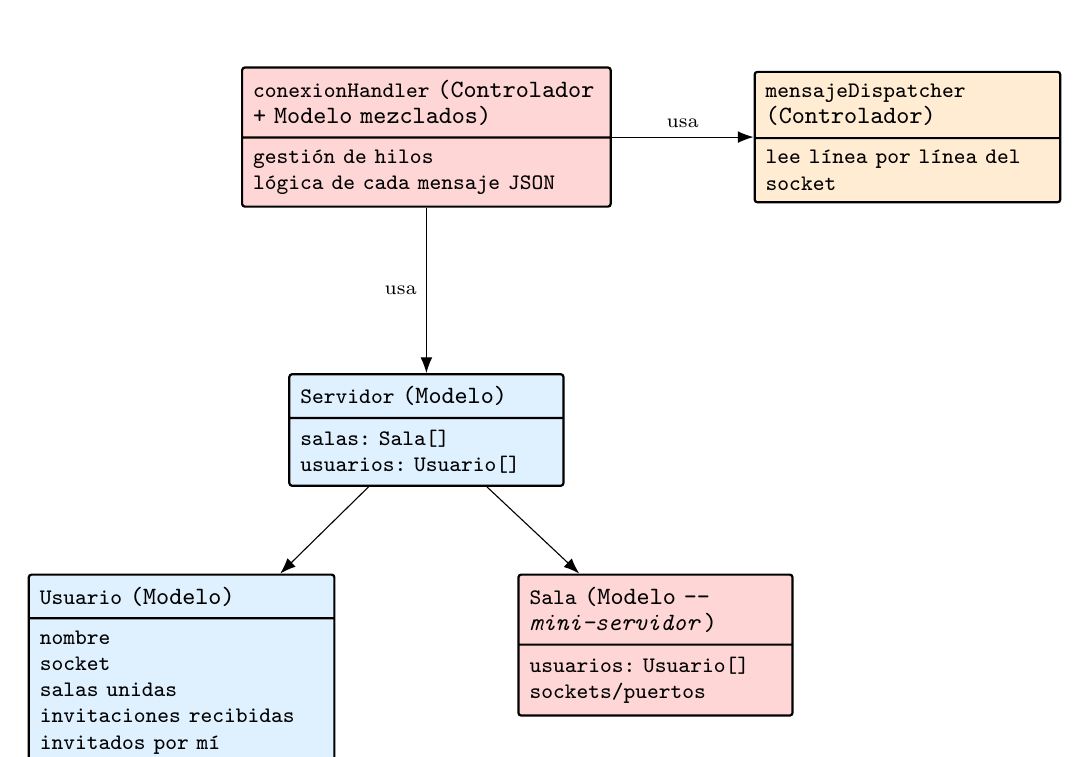
\begin{tikzpicture}[node distance=1.1cm and 1.6cm]

\classbox{Servidor}{cajamodelo}{3.2cm}{}
  {\textbf{Servidor} \small(Modelo)
   \nodepart{two} salas: Sala[] \\ usuarios: Usuario[]};

\classbox{Usuario}{cajamodelo}{3.6cm}{below left=1.1cm and -0.6cm of Servidor}
  {\textbf{Usuario} \small(Modelo)
   \nodepart{two} nombre \\ socket \\ salas unidas \\ invitaciones recibidas \\ invitados por mí};

\classbox{Sala}{cajaproblema}{3.2cm}{below right=1.1cm and -0.6cm of Servidor}
  {\textbf{Sala} \small(Modelo -- \emph{mini-servidor})
   \nodepart{two} usuarios: Usuario[] \\ sockets/puertos};

\classbox{Conexion}{cajaproblema}{4.4cm}{above=2.1cm of Servidor}
  {\textbf{conexionHandler} \small(Controlador + Modelo mezclados)
   \nodepart{two} gestión de hilos \\ lógica de cada mensaje JSON};

\classbox{Dispatcher}{cajacontrol}{3.6cm}{right=1.8cm of Conexion}
  {\textbf{mensajeDispatcher} \small(Controlador)
   \nodepart{two} lee línea por línea del socket};

\draw[-{Latex[length=2mm]}] (Servidor) -- (Usuario);
\draw[-{Latex[length=2mm]}] (Servidor) -- (Sala);
\draw[-{Latex[length=2mm]}] (Conexion) -- node[left,font=\scriptsize]{usa} (Servidor);
\draw[-{Latex[length=2mm]}] (Conexion) -- node[above,font=\scriptsize]{usa} (Dispatcher);

\end{tikzpicture}
\caption{Diseño original de la primera iteración (en C). En rojo, los dos
puntos que el propio proceso de desarrollo identificó como errores de
diseño: \texttt{Sala} concebida como un mini-servidor redundante, y
\texttt{conexionHandler} mezclando responsabilidades de Controlador y de
Modelo.}
\label{fig:diagrama-c}
\end{figure}

Más allá del diseño, las dificultades \emph{de implementación} en C fueron
determinantes para abandonar esta versión:

\begin{itemize}
  \item \textbf{Simular objetos.} C no tiene encapsulación real; las
        "clases" se simularon con \emph{structs} y referencias en memoria,
        y cada "clase" debía diseñarse por completo en su archivo de
        cabecera antes de poder escribir una sola línea de su
        implementación, lo que hacía el ciclo de desarrollo mucho más
        lento que en un lenguaje orientado a objetos.
  \item \textbf{JSON en C.} Existen bibliotecas de parseo de JSON para C,
        pero ninguna resuelve el problema por completo: sin importar cuánto
        trabajo ahorre la biblioteca, seguía siendo necesario escribir a
        mano una cantidad considerable de código para cumplir el protocolo
        al pie de la letra.
  \item \textbf{Hilos y memoria compartida.} Evitar que dos hilos alteraran
        el mismo lugar en memoria al mismo tiempo se resolvió con mutex de
        \texttt{pthreads}, pero administrar manualmente cuándo bloquear y
        desbloquear cada recurso resultó, con mucho, la parte más difícil
        de todo el proyecto.
  \item \textbf{Pruebas.} Contrario a lo anterior, escribir pruebas
        unitarias fue relativamente sencillo gracias a la biblioteca
        \texttt{cmocka}, que funcionó bien para este propósito.
\end{itemize}

La combinación de manejo manual de memoria, bibliotecas de JSON
incompletas y sincronización de hilos de bajo nivel hizo que el desarrollo
avanzara muy lento; ante la falta de tiempo, se tomó la decisión de
descartar por completo la versión en C y reiniciar el proyecto en C\#,
decisión que se retoma con más detalle en las Conclusiones.

\subsection{Segunda iteración: diseño final en C\#}

La versión que finalmente se entrega aplica directamente las lecciones de
la primera iteración. Se organizó en \textbf{tres proyectos} de .NET
(figura~\ref{fig:arquitectura-general}): \texttt{server} y
\texttt{client}, cada uno con su propio Modelo, Vista y Controlador; y
\texttt{chatComun}, una biblioteca compartida que contiene únicamente el
código de bajo nivel que \emph{ambos} programas necesitan de forma
idéntica —partir el flujo de bytes en líneas y serializar/leer JSON—, de
modo que esa lógica no se duplique en dos lugares distintos como habría
ocurrido de seguir separando el proyecto en solo dos partes.

\begin{figure}[H]
\centering
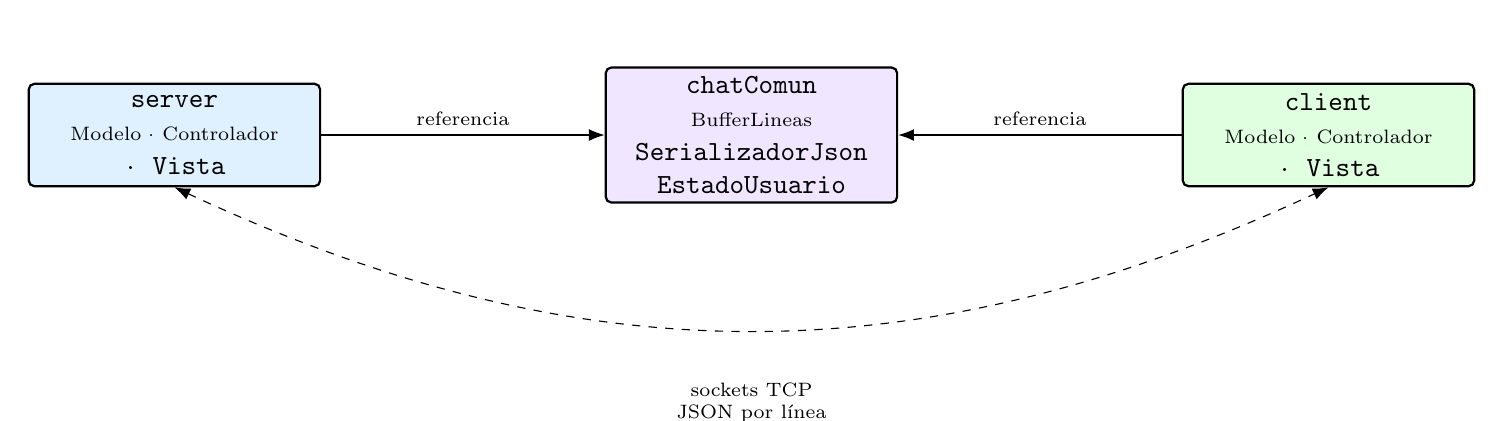
\begin{tikzpicture}[node distance=2.6cm]
\node[rectangle, draw=black, thick, rounded corners=2pt, fill=cajacomun,
      font=\bfseries\ttfamily, minimum width=3.7cm, minimum height=1.3cm,
      align=center] (comun) {chatComun\\\scriptsize\normalfont\upshape BufferLineas\\ SerializadorJson\\ EstadoUsuario};
\node[rectangle, draw=black, thick, rounded corners=2pt, fill=cajamodelo,
      font=\bfseries\ttfamily, minimum width=3.7cm, minimum height=1.3cm,
      align=center, left=3.6cm of comun] (server) {server\\\scriptsize\normalfont\upshape Modelo · Controlador\\ · Vista};
\node[rectangle, draw=black, thick, rounded corners=2pt, fill=cajavista,
      font=\bfseries\ttfamily, minimum width=3.7cm, minimum height=1.3cm,
      align=center, right=3.6cm of comun] (client) {client\\\scriptsize\normalfont\upshape Modelo · Controlador\\ · Vista};
\draw[-{Latex[length=2mm]}] (server) -- node[above,font=\scriptsize]{referencia} (comun);
\draw[-{Latex[length=2mm]}] (client) -- node[above,font=\scriptsize]{referencia} (comun);
\draw[{Latex[length=2mm]}-{Latex[length=2mm]}, dashed]
  (server.south) to[bend right=25]
  node[below=0.55cm, font=\scriptsize, align=center] {sockets TCP\\JSON por línea}
  (client.south);
\end{tikzpicture}
\caption{Arquitectura general: dos programas independientes que comparten
únicamente el código de bajo nivel del protocolo a través de
\texttt{chatComun}.}
\label{fig:arquitectura-general}
\end{figure}

\subsubsection*{Diagrama de clases del servidor}

\begin{figure}[H]
\centering
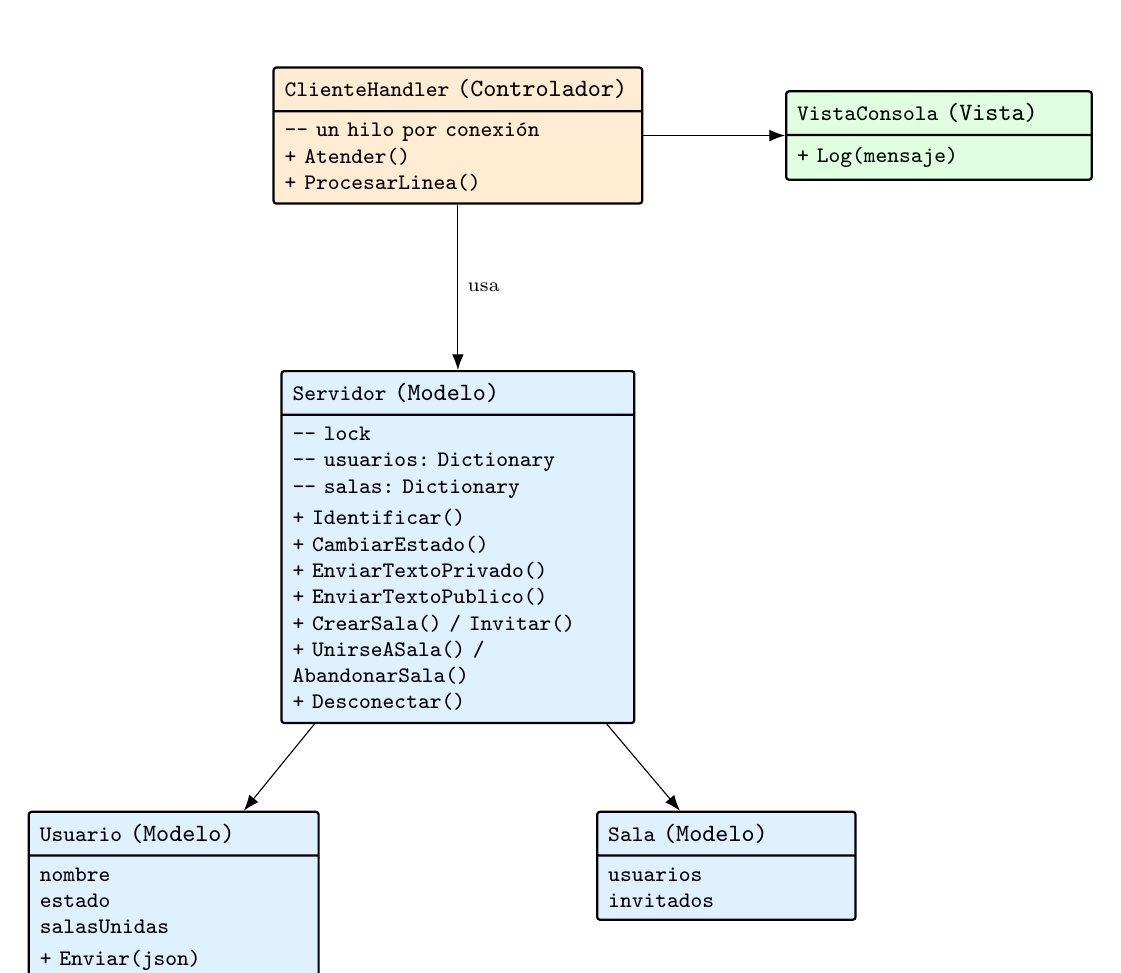
\begin{tikzpicture}[node distance=1.0cm and 1.5cm]

\classbox{ServidorCS}{cajamodelo}{4.2cm}{}
  {\textbf{Servidor} \small(Modelo)
   \nodepart{two}
   -- lock \\
   -- usuarios: Dictionary \\
   -- salas: Dictionary
   \\[2pt]
   + Identificar() \\
   + CambiarEstado() \\
   + EnviarTextoPrivado() \\
   + EnviarTextoPublico() \\
   + CrearSala() / Invitar() \\
   + UnirseASala() / AbandonarSala() \\
   + Desconectar()};

\classbox{UsuarioCS}{cajamodelo}{3.4cm}{below left=1.1cm and -0.5cm of ServidorCS}
  {\textbf{Usuario} \small(Modelo)
   \nodepart{two}
   nombre \\ estado \\ salasUnidas
   \\[2pt] + Enviar(json)};

\classbox{SalaCS}{cajamodelo}{3.0cm}{below right=1.1cm and -0.5cm of ServidorCS}
  {\textbf{Sala} \small(Modelo)
   \nodepart{two}
   usuarios \\ invitados};

\classbox{HandlerCS}{cajacontrol}{4.4cm}{above=2.1cm of ServidorCS}
  {\textbf{ClienteHandler} \small(Controlador)
   \nodepart{two}
   -- un hilo por conexión \\
   + Atender() \\
   + ProcesarLinea()};

\classbox{VistaCS}{cajavista}{3.6cm}{right=1.8cm of HandlerCS}
  {\textbf{VistaConsola} \small(Vista)
   \nodepart{two} + Log(mensaje)};

\draw[-{Latex[length=2mm]}] (ServidorCS) -- (UsuarioCS);
\draw[-{Latex[length=2mm]}] (ServidorCS) -- (SalaCS);
\draw[-{Latex[length=2mm]}] (HandlerCS) -- node[right,font=\scriptsize]{usa} (ServidorCS);
\draw[-{Latex[length=2mm]}] (HandlerCS) -- (VistaCS);

\end{tikzpicture}
\caption{Servidor en C\#: \texttt{Servidor} concentra toda la lógica de
negocio y la sincronización con un único candado; \texttt{ClienteHandler}
es un controlador delgado, uno por conexión, que solo traduce JSON en
llamadas al Modelo. \texttt{Usuario} y \texttt{Sala} ya no intentan actuar
como servidores por su cuenta: toda la membresía se resuelve de forma
centralizada, corrigiendo el problema señalado en la
figura~\ref{fig:diagrama-c}.}
\label{fig:diagrama-servidor-cs}
\end{figure}

\subsubsection*{Diagrama de clases del cliente}

\begin{figure}[H]
\centering
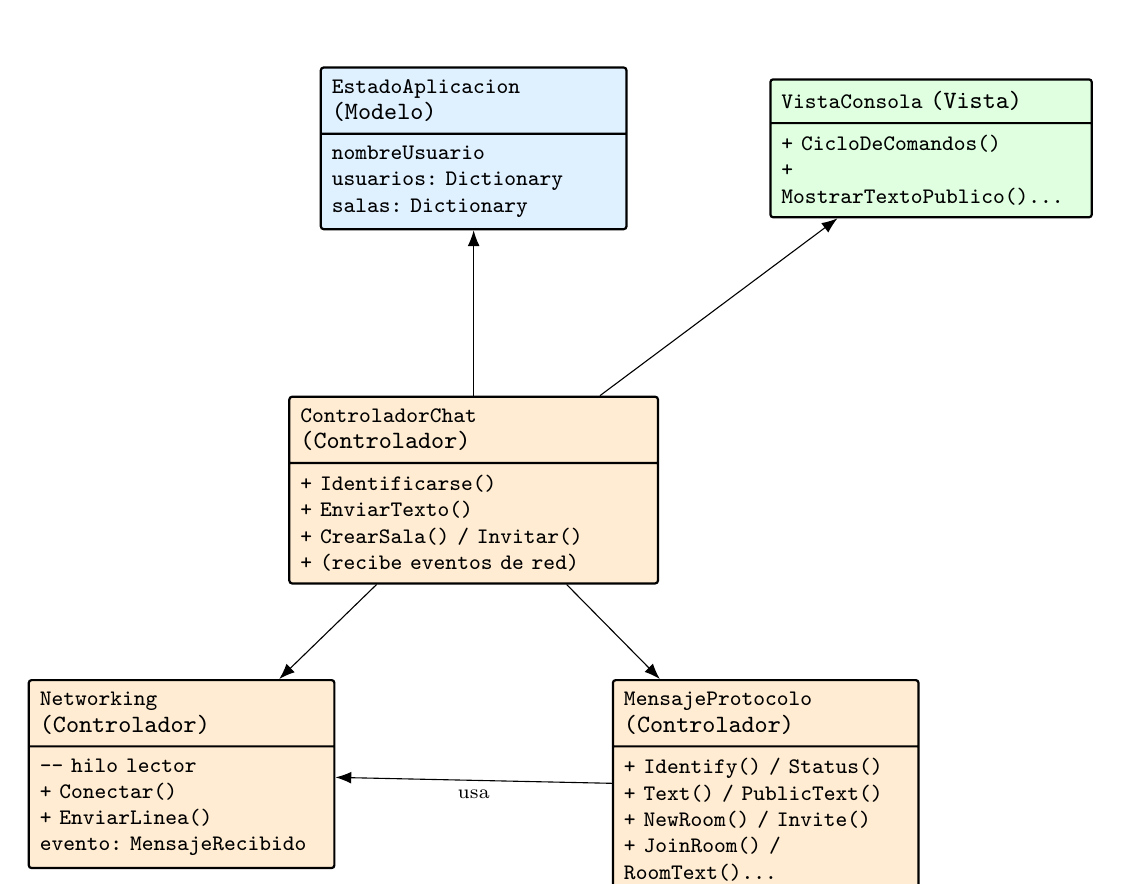
\begin{tikzpicture}[node distance=1.0cm and 1.4cm]

\classbox{ControladorCS}{cajacontrol}{4.4cm}{}
  {\textbf{ControladorChat} \small(Controlador)
   \nodepart{two}
   + Identificarse() \\
   + EnviarTexto() \\
   + CrearSala() / Invitar() \\
   + (recibe eventos de red)};

\classbox{NetCS}{cajacontrol}{3.6cm}{below left=1.2cm and -0.6cm of ControladorCS}
  {\textbf{Networking} \small(Controlador)
   \nodepart{two}
   -- hilo lector \\
   + Conectar() \\
   + EnviarLinea() \\
   evento: MensajeRecibido};

\classbox{ProtoCS}{cajacontrol}{3.6cm}{below right=1.2cm and -0.6cm of ControladorCS}
  {\textbf{MensajeProtocolo} \small(Controlador)
   \nodepart{two}
   + Identify() / Status() \\
   + Text() / PublicText() \\
   + NewRoom() / Invite() \\
   + JoinRoom() / RoomText()...};

\classbox{EstadoCS}{cajamodelo}{3.6cm}{above=2.1cm of ControladorCS}
  {\textbf{EstadoAplicacion} \small(Modelo)
   \nodepart{two}
   nombreUsuario \\ usuarios: Dictionary \\ salas: Dictionary};

\classbox{VistaClienteCS}{cajavista}{3.8cm}{right=1.8cm of EstadoCS}
  {\textbf{VistaConsola} \small(Vista)
   \nodepart{two}
   + CicloDeComandos() \\
   + MostrarTextoPublico()...};

\draw[-{Latex[length=2mm]}] (ControladorCS) -- (NetCS);
\draw[-{Latex[length=2mm]}] (ControladorCS) -- (ProtoCS);
\draw[-{Latex[length=2mm]}] (ProtoCS) -- node[below,font=\scriptsize]{usa} (NetCS);
\draw[-{Latex[length=2mm]}] (ControladorCS) -- (EstadoCS);
\draw[-{Latex[length=2mm]}] (ControladorCS) -- (VistaClienteCS);

\end{tikzpicture}
\caption{Cliente en C\#: \texttt{Networking} es la clase dedicada
exclusivamente a la conexión TCP; \texttt{MensajeProtocolo} construye cada
mensaje del protocolo y lo envía a través de \texttt{Networking};
\texttt{ControladorChat} conecta ambas con el Modelo
(\texttt{EstadoAplicacion}) y la Vista.}
\label{fig:diagrama-cliente-cs}
\end{figure}

\subsubsection*{Ejemplo de flujo: \texttt{IDENTIFY}}

La figura~\ref{fig:secuencia-identify} ilustra por qué el hilo por conexión
y el candado del servidor son necesarios incluso para la operación más
simple del protocolo: identificar a un usuario debe, de forma atómica,
revisar que el nombre no exista y registrarlo, y además debe notificarle a
\emph{todos los demás} clientes conectados —cada uno atendido por su propio
hilo— sin que dos identificaciones simultáneas dejen la tabla de usuarios
en un estado inconsistente.

\begin{figure}[H]
\centering
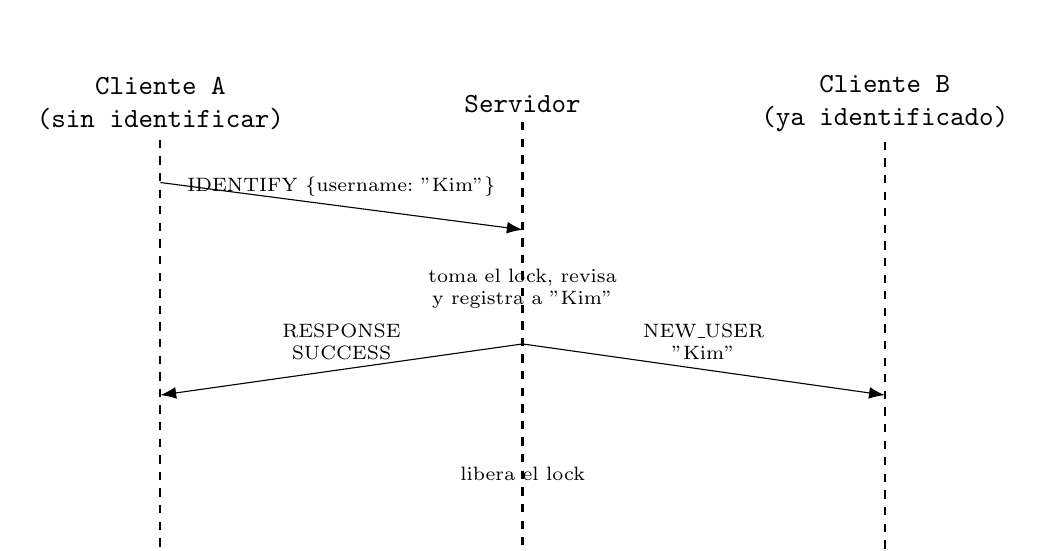
\begin{tikzpicture}[
  actor/.style={font=\bfseries\ttfamily, align=center},
  lifeline/.style={dashed, thick},
  msg/.style={-{Latex[length=2mm]}, font=\scriptsize}
]
\node[actor] (A) at (0,0) {Cliente A\\(sin identificar)};
\node[actor] (S) at (4.6,0) {Servidor};
\node[actor] (B) at (9.2,0) {Cliente B\\(ya identificado)};

\draw[lifeline] (A) -- ++(0,-5.8);
\draw[lifeline] (S) -- ++(0,-5.8);
\draw[lifeline] (B) -- ++(0,-5.8);

\draw[msg] (0,-1) -- node[above,text width=4.2cm,align=center]{IDENTIFY \{username: "Kim"\}} (4.6,-1.6);
\node[font=\scriptsize, align=center, text width=4.6cm] at (4.6,-2.35) {toma el lock, revisa\\y registra a "Kim"};
\draw[msg] (4.6,-3.05) -- node[above,text width=3cm,align=center]{RESPONSE\\SUCCESS} (0,-3.7);
\draw[msg] (4.6,-3.05) -- node[above,text width=3cm,align=center]{NEW\_USER\\"Kim"} (9.2,-3.7);
\node[font=\scriptsize] at (4.6,-4.7) {libera el lock};

\end{tikzpicture}
\caption{Al identificarse, el servidor responde solo a quien lo pidió, pero
además difunde \texttt{NEW\_USER} a todos los demás clientes ya conectados,
cada uno en su propio hilo; el candado global garantiza que ninguna otra
identificación concurrente vea la tabla de usuarios a medio actualizar.}
\label{fig:secuencia-identify}
\end{figure}

\subsection{Trazabilidad protocolo -- código}

La tabla~\ref{tab:trazabilidad} muestra, para cada mensaje que el servidor
recibe, el método del Modelo que implementa la regla de negocio y el punto
del Controlador que lo invoca, dejando explícita la correspondencia entre
la especificación y la implementación.

\begin{longtable}{@{}p{2.3cm}p{5.2cm}p{5.5cm}@{}}
\toprule
\textbf{Mensaje} & \textbf{Método en \texttt{Servidor} (Modelo)} & \textbf{Manejador en \texttt{ClienteHandler} (Controlador)} \\
\midrule
\endhead
\texttt{IDENTIFY} & \texttt{Identificar(Usuario)} & \texttt{ManejarIdentify} \\
\texttt{STATUS} & \texttt{CambiarEstado(Usuario, Estado)} & \texttt{ManejarStatus} \\
\texttt{USERS} & \texttt{ObtenerUsuarios()} & \texttt{ManejarUsers} \\
\texttt{TEXT} & \texttt{EnviarTextoPrivado(...)} & \texttt{ManejarText} \\
\texttt{PUBLIC\_TEXT} & \texttt{EnviarTextoPublico(...)} & \texttt{ManejarPublicText} \\
\texttt{NEW\_ROOM} & \texttt{CrearSala(...)} & \texttt{ManejarNewRoom} \\
\texttt{INVITE} & \texttt{Invitar(...)} & \texttt{ManejarInvite} \\
\texttt{JOIN\_ROOM} & \texttt{UnirseASala(...)} & \texttt{ManejarJoinRoom} \\
\texttt{ROOM\_USERS} & \texttt{ObtenerUsuariosDeSala(...)} & \texttt{ManejarRoomUsers} \\
\texttt{ROOM\_TEXT} & \texttt{EnviarTextoSala(...)} & \texttt{ManejarRoomText} \\
\texttt{LEAVE\_ROOM} & \texttt{AbandonarSala(...)} & \texttt{ManejarLeaveRoom} \\
\texttt{DISCONNECT} & \texttt{Desconectar(Usuario)} & (cierre de conexión en \texttt{Atender}) \\
\bottomrule
\caption{Cada operación del protocolo tiene un único método responsable en
el Modelo; el Controlador nunca decide reglas de negocio por su cuenta,
corrigiendo así el problema de diseño de \texttt{conexionHandler} en la
primera iteración.}
\label{tab:trazabilidad}
\end{longtable}

% ==============================================================
\section{Implementación}
% ==============================================================

\subsection{Tecnologías utilizadas}

\begin{itemize}
  \item \textbf{Lenguaje y runtime:} C\# 12 sobre .NET 8 (LTS), tanto para
        el servidor como para el cliente.
  \item \textbf{Sockets:} \texttt{System.Net.Sockets.TcpListener} en el
        servidor para aceptar conexiones, y \texttt{TcpClient} /
        \texttt{NetworkStream} en ambos programas para leer y escribir el
        flujo de bytes.
  \item \textbf{Concurrencia:} \texttt{System.Threading.Thread} —un hilo
        por conexión aceptada en el servidor, y un hilo lector en segundo
        plano en el cliente— junto con la instrucción \texttt{lock} de C\#
        (basada en \texttt{Monitor}) para proteger el estado compartido del
        servidor.
  \item \textbf{JSON:} \texttt{System.Text.Json}, incluida en el propio
        runtime de .NET; no se agregó ningún paquete NuGet externo al
        proyecto.
  \item \textbf{Organización del código:} tres proyectos de .NET
        (\texttt{chatComun}, \texttt{server}, \texttt{client})
        reunidos en una sola solución (\texttt{ChatMulti.sln}).
\end{itemize}

\subsection{Requisitos para ejecutar el proyecto}

\begin{itemize}
  \item SDK de \textbf{.NET 8} instalado (funciona igual en Linux, Windows
        o macOS).
  \item Para probar el chat entre dos máquinas distintas: ambas conectadas
        a la \emph{misma} red local, con el puerto elegido para el
        servidor permitido en el firewall de la máquina que hace de
        servidor (por ejemplo, con \texttt{ufw allow <puerto>/tcp} en
        distribuciones basadas en Debian/Ubuntu).
\end{itemize}

\subsection{Instrucciones de compilación y ejecución}

\begin{verbatim}
# Desde la carpeta raíz del proyecto (donde está ChatMulti.sln):
dotnet build ChatMulti.sln

# Terminal 1: servidor (el puerto es opcional; por defecto 5000)
dotnet run --project server -- 5000

# Terminal 2, 3, ... : un cliente por cada usuario que se quiera conectar
dotnet run --project client
\end{verbatim}

Al arrancar, el cliente pregunta de forma interactiva el \emph{host}
(dirección IP del servidor, o \texttt{localhost} si ambos corren en la
misma máquina), el puerto, y el nombre de usuario con el que se desea
identificar. Una vez conectado, se escribe texto público directamente, o
se usan comandos con prefijo \texttt{/} para el resto de las operaciones
del protocolo (\texttt{/status}, \texttt{/msg}, \texttt{/newroom},
\texttt{/invite}, \texttt{/join}, \texttt{/roomusers}, \texttt{/roomtext},
\texttt{/leave}, \texttt{/quit}).

\subsection{Estado de las pruebas}

En la primera iteración (en C) sí se llegaron a escribir pruebas unitarias
con la biblioteca \texttt{cmocka}, y funcionaron bien para ese propósito.
Por restricciones de tiempo, esas pruebas \textbf{no} se portaron a la
versión final en C\#; queda como trabajo inmediato agregar un proyecto de
pruebas (por ejemplo con xUnit) para \texttt{chatComun} y para la clase
\texttt{Servidor}, que al no depender de sockets reales se puede probar
de forma aislada.

% ==============================================================
\section{Conclusiones}
% ==============================================================

El mayor reto de todo el proyecto fue, sin duda, la programación
concurrente —en particular durante la primera iteración en C, donde
sincronizar hilos con mutex de bajo nivel y, al mismo tiempo, administrar
memoria manualmente, resultó abrumador—. Pasar a C\# no eliminó la
necesidad de razonar cuidadosamente sobre concurrencia, pero sí quitó de
en medio dos fuentes constantes de errores (la gestión manual de memoria y
la simulación de objetos con \emph{structs} y cabeceras), dejando espacio
para concentrarse en el problema real: qué estado compartir y cómo
protegerlo.

Escribir pruebas unitarias en C con \texttt{cmocka} fue, de hecho, una de
las partes más sencillas y más valiosas del proceso: obligó a pensar en
casos límite del protocolo desde antes de que aparecieran como bugs en
producción, y es una práctica que se pretende retomar en C\# como
siguiente paso. De manera relacionada, el proyecto dejó claro que la
primera versión de un programa rara vez es la definitiva, y que reconocer a
tiempo cuándo conviene desechar un diseño (o una implementación completa,
como ocurrió con la versión en C) y empezar de nuevo es tan importante
como saber cuándo seguir insistiendo.

Esta fue también la primera vez que se usó \texttt{git} de forma seria
para llevar el desarrollo; aunque nunca fue necesario recurrir a una
versión anterior estable, tener ese respaldo disponible en todo momento dio
mucha más tranquilidad para experimentar y refactorizar sin miedo a perder
trabajo.

\subsection*{Posibles mejoras}

\begin{itemize}
  \item Agregar manejo de errores más claro en el cliente al fallar la
        conexión inicial (por ejemplo, distinguir un \emph{timeout} de una
        conexión rechazada, en vez de una excepción genérica).
  \item Portar las pruebas unitarias de la versión en C a un proyecto de
        pruebas para la versión en C\#.
  \item Si el protocolo creciera, migrar de objetos JSON dinámicos a
        clases (DTOs) fuertemente tipadas por cada tipo de mensaje.
\end{itemize}

\subsection*{Trabajo futuro / posible expansión}

\begin{itemize}
  \item \textbf{Autenticación:} permitir contraseñas o algún otro mecanismo
        para evitar que cualquiera se identifique con el nombre de otro
        usuario disponible.
  \item \textbf{Cifrado:} envolver la conexión TCP con TLS, para que los
        mensajes no viajen en texto plano dentro de la red local.
  \item \textbf{Privacidad de IPs:} evitar que quien tenga acceso al
        servidor pueda ver trivialmente la dirección IP de cada usuario
        conectado.
  \item \textbf{Escalabilidad:} para soportar mucho más allá de la decena
        de miles de usuarios concurrentes contemplados en el alcance,
        explorar múltiples instancias de servidor coordinadas por un
        sistema de mensajería (por ejemplo, un \emph{message broker}), en
        vez de un único proceso con estado en memoria.
  \item \textbf{Interfaz gráfica:} gracias a haber seguido MVC, sustituir
        \texttt{VistaConsola} por una interfaz gráfica (WPF, Avalonia, o
        incluso una aplicación web) no debería requerir tocar el Modelo ni
        el Controlador del cliente.
\end{itemize}

% ==============================================================
\section{Bibliografía}
% ==============================================================

\begin{itemize}
  \item Protocolo del chat multiusuario, documento proporcionado por el
        profesor (Canek) en el curso \emph{Modelado y Programación}
        (material de curso, sin publicar).
  \item Microsoft. \emph{System.Text.Json Namespace}. Documentación de la
        API de .NET.
        \url{https://learn.microsoft.com/en-us/dotnet/api/system.text.json}
  \item Microsoft. \emph{TcpListener Class}. Documentación de la API de
        .NET.
        \url{https://learn.microsoft.com/en-us/dotnet/api/system.net.sockets.tcplistener}
  \item Microsoft. \emph{TcpClient Class}. Documentación de la API de
        .NET.
        \url{https://learn.microsoft.com/en-us/dotnet/api/system.net.sockets.tcpclient}
  \item Microsoft. \emph{Thread Class}. Documentación de la API de .NET.
        \url{https://learn.microsoft.com/en-us/dotnet/api/system.threading.thread}
  \item Microsoft. \emph{The lock statement -- ensure exclusive access to a
        shared resource}. Referencia del lenguaje C\#.
        \url{https://learn.microsoft.com/en-us/dotnet/csharp/language-reference/statements/lock}
  \item cmocka. \emph{cmocka -- unit testing framework for C}.
        \url{https://cmocka.org/}
\end{itemize}

\end{document}
